\documentclass[twoside]{book}

% Packages required by doxygen
\usepackage{fixltx2e}
\usepackage{calc}
\usepackage{doxygen}
\usepackage[export]{adjustbox} % also loads graphicx
\usepackage{graphicx}
\usepackage[utf8]{inputenc}
\usepackage{makeidx}
\usepackage{multicol}
\usepackage{multirow}
\PassOptionsToPackage{warn}{textcomp}
\usepackage{textcomp}
\usepackage[nointegrals]{wasysym}
\usepackage[table]{xcolor}

% Font selection
\usepackage[T1]{fontenc}
\usepackage[scaled=.90]{helvet}
\usepackage{courier}
\usepackage{amssymb}
\usepackage{sectsty}
\renewcommand{\familydefault}{\sfdefault}
\allsectionsfont{%
  \fontseries{bc}\selectfont%
  \color{darkgray}%
}
\renewcommand{\DoxyLabelFont}{%
  \fontseries{bc}\selectfont%
  \color{darkgray}%
}
\newcommand{\+}{\discretionary{\mbox{\scriptsize$\hookleftarrow$}}{}{}}

% Page & text layout
\usepackage{geometry}
\geometry{%
  a4paper,%
  top=2.5cm,%
  bottom=2.5cm,%
  left=2.5cm,%
  right=2.5cm%
}
\tolerance=750
\hfuzz=15pt
\hbadness=750
\setlength{\emergencystretch}{15pt}
\setlength{\parindent}{0cm}
\setlength{\parskip}{3ex plus 2ex minus 2ex}
\makeatletter
\renewcommand{\paragraph}{%
  \@startsection{paragraph}{4}{0ex}{-1.0ex}{1.0ex}{%
    \normalfont\normalsize\bfseries\SS@parafont%
  }%
}
\renewcommand{\subparagraph}{%
  \@startsection{subparagraph}{5}{0ex}{-1.0ex}{1.0ex}{%
    \normalfont\normalsize\bfseries\SS@subparafont%
  }%
}
\makeatother

% Headers & footers
\usepackage{fancyhdr}
\pagestyle{fancyplain}
\fancyhead[LE]{\fancyplain{}{\bfseries\thepage}}
\fancyhead[CE]{\fancyplain{}{}}
\fancyhead[RE]{\fancyplain{}{\bfseries\leftmark}}
\fancyhead[LO]{\fancyplain{}{\bfseries\rightmark}}
\fancyhead[CO]{\fancyplain{}{}}
\fancyhead[RO]{\fancyplain{}{\bfseries\thepage}}
\fancyfoot[LE]{\fancyplain{}{}}
\fancyfoot[CE]{\fancyplain{}{}}
\fancyfoot[RE]{\fancyplain{}{\bfseries\scriptsize Generated by Doxygen }}
\fancyfoot[LO]{\fancyplain{}{\bfseries\scriptsize Generated by Doxygen }}
\fancyfoot[CO]{\fancyplain{}{}}
\fancyfoot[RO]{\fancyplain{}{}}
\renewcommand{\footrulewidth}{0.4pt}
\renewcommand{\chaptermark}[1]{%
  \markboth{#1}{}%
}
\renewcommand{\sectionmark}[1]{%
  \markright{\thesection\ #1}%
}

% Indices & bibliography
\usepackage{natbib}
\usepackage[titles]{tocloft}
\setcounter{tocdepth}{3}
\setcounter{secnumdepth}{5}
\makeindex

% Hyperlinks (required, but should be loaded last)
\usepackage{ifpdf}
\ifpdf
  \usepackage[pdftex,pagebackref=true]{hyperref}
\else
  \usepackage[ps2pdf,pagebackref=true]{hyperref}
\fi
\hypersetup{%
  colorlinks=true,%
  linkcolor=blue,%
  citecolor=blue,%
  unicode%
}

% Custom commands
\newcommand{\clearemptydoublepage}{%
  \newpage{\pagestyle{empty}\cleardoublepage}%
}

\usepackage{caption}
\captionsetup{labelsep=space,justification=centering,font={bf},singlelinecheck=off,skip=4pt,position=top}

%===== C O N T E N T S =====

\begin{document}

% Titlepage & ToC
\hypersetup{pageanchor=false,
             bookmarksnumbered=true,
             pdfencoding=unicode
            }
\pagenumbering{alph}
\begin{titlepage}
\vspace*{7cm}
\begin{center}%
{\Large R\+N\+A\+Red\+Print }\\
\vspace*{1cm}
{\large Generated by Doxygen 1.8.13}\\
\end{center}
\end{titlepage}
\clearemptydoublepage
\pagenumbering{roman}
\tableofcontents
\clearemptydoublepage
\pagenumbering{arabic}
\hypersetup{pageanchor=true}

%--- Begin generated contents ---
\chapter{Hierarchical Index}
\section{Class Hierarchy}
This inheritance list is sorted roughly, but not completely, alphabetically\+:\begin{DoxyCompactList}
\item \contentsline{section}{Bag}{\pageref{class_bag}}{}
\item \contentsline{section}{Base\+Pair}{\pageref{class_base_pair}}{}
\item \contentsline{section}{Loop}{\pageref{class_loop}}{}
\item \contentsline{section}{Secondary\+Structure}{\pageref{class_secondary_structure}}{}
\item \contentsline{section}{Tree\+Decomposition}{\pageref{class_tree_decomposition}}{}
\item \contentsline{section}{Tree\+Decomposition\+Factory}{\pageref{class_tree_decomposition_factory}}{}
\begin{DoxyCompactList}
\item \contentsline{section}{T\+D\+Lib\+Factory}{\pageref{class_t_d_lib_factory}}{}
\end{DoxyCompactList}
\end{DoxyCompactList}

\chapter{Class Index}
\section{Class List}
Here are the classes, structs, unions and interfaces with brief descriptions\+:\begin{DoxyCompactList}
\item\contentsline{section}{\hyperlink{class_bag}{Bag} \\*Set of indices, ie positions in the sequences that must be jointly considered in the context of a given tree-\/decomposition }{\pageref{class_bag}}{}
\item\contentsline{section}{\hyperlink{class_base_pair}{Base\+Pair} \\*Encodes a basic base pair }{\pageref{class_base_pair}}{}
\item\contentsline{section}{\hyperlink{class_loop}{Loop} \\*\hyperlink{class_loop}{Loop} in the Turner model, ie a set of indices }{\pageref{class_loop}}{}
\item\contentsline{section}{\hyperlink{class_secondary_structure}{Secondary\+Structure} \\*R\+NA secondary structure, possibly with pseudoknots }{\pageref{class_secondary_structure}}{}
\item\contentsline{section}{\hyperlink{class_t_d_lib_factory}{T\+D\+Lib\+Factory} \\*Concrete implementation of \hyperlink{class_tree_decomposition_factory}{Tree\+Decomposition\+Factory} based on the T\+D\+Lib.\+jar Java implementation of the greedy fill-\/in heuristics }{\pageref{class_t_d_lib_factory}}{}
\item\contentsline{section}{\hyperlink{class_tree_decomposition}{Tree\+Decomposition} }{\pageref{class_tree_decomposition}}{}
\item\contentsline{section}{\hyperlink{class_tree_decomposition_factory}{Tree\+Decomposition\+Factory} \\*Abstract class aimed at producing a tree decomposition from a set of secondary structures }{\pageref{class_tree_decomposition_factory}}{}
\end{DoxyCompactList}

\chapter{Class Documentation}
\hypertarget{class_bag}{}\section{Bag Class Reference}
\label{class_bag}\index{Bag@{Bag}}


The \hyperlink{class_bag}{Bag} class represents a set of indices, ie positions in the sequences that must be jointly considered in the context of a given tree-\/decomposition.  




{\ttfamily \#include $<$Tree\+Decomposition.\+hpp$>$}



Collaboration diagram for Bag\+:\nopagebreak
\begin{figure}[H]
\begin{center}
\leavevmode
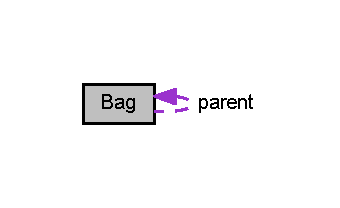
\includegraphics[width=163pt]{class_bag__coll__graph}
\end{center}
\end{figure}
\subsection*{Public Member Functions}
\begin{DoxyCompactItemize}
\item 
\hyperlink{class_bag_aaa75e2de63f2f6199973471491cb9e13}{Bag} (int i)
\begin{DoxyCompactList}\small\item\em \hyperlink{class_bag}{Bag} Constructs a bag with given identifier. \end{DoxyCompactList}\item 
void \hyperlink{class_bag_a4f5fcc1b48aeb967653a0d5364254562}{add\+Index} (int i)
\begin{DoxyCompactList}\small\item\em add\+Index Adds an index/position to this bag \end{DoxyCompactList}\item 
vector$<$ int $>$ \hyperlink{class_bag_ad05a3a0069514372df097ec7d0cbe638}{get\+Indices} ()
\begin{DoxyCompactList}\small\item\em get\+Indices Returns the set of indices/positions for this bag \end{DoxyCompactList}\item 
void \hyperlink{class_bag_a8dfb102ead7412437b5f69b582784e44}{order\+Indices} ()
\begin{DoxyCompactList}\small\item\em order\+Indices Reorders the indices such that the proper index is put at the last position in the index list. \end{DoxyCompactList}\item 
void \hyperlink{class_bag_a36747193c7212f45b68552c3ea31fd70}{add\+Child} (\hyperlink{class_bag}{Bag} $\ast$b)
\begin{DoxyCompactList}\small\item\em add\+Child Adds a child to the bag \end{DoxyCompactList}\item 
void \hyperlink{class_bag_ade9c24ae6e76c2e0c27bc5b51929f64a}{replace\+Child} (\hyperlink{class_bag}{Bag} $\ast$prev, \hyperlink{class_bag}{Bag} $\ast$next)
\begin{DoxyCompactList}\small\item\em replace\+Child Replaces any occurrence of a bag in the list of children bags with another bag \end{DoxyCompactList}\item 
void \hyperlink{class_bag_a44101c6b26782dbe076d51e77f35ce81}{set\+Parent} (\hyperlink{class_bag}{Bag} $\ast$b)
\begin{DoxyCompactList}\small\item\em set\+Parent Sets the parent of this bag to a given bag \end{DoxyCompactList}\item 
int \hyperlink{class_bag_a03b31223756e1f3d7c040a72e53597d7}{num\+Proper} ()
\begin{DoxyCompactList}\small\item\em num\+Proper Returns the number of proper indices for this bag \end{DoxyCompactList}\item 
vector$<$ int $>$ \hyperlink{class_bag_a84860e8af1eed9547b7c20d77d29da7d}{get\+Proper\+Indices} ()
\begin{DoxyCompactList}\small\item\em get\+Proper\+Indices Returns the list of proper indices for this bag \end{DoxyCompactList}\item 
vector$<$ \hyperlink{class_bag}{Bag} $\ast$ $>$ \hyperlink{class_bag_a79094c130b1fd55e49afeeafa70c454b}{get\+Children} ()
\begin{DoxyCompactList}\small\item\em get\+Children Returns the list of children bags for this bag \end{DoxyCompactList}\item 
vector$<$ int $>$ \hyperlink{class_bag_a1a7660f8e31d6941fdec07c86e0fe3ac}{get\+Proper\+Parent\+Indices} ()
\begin{DoxyCompactList}\small\item\em get\+Proper\+Parent\+Indices Returns the list of indices that are proper to the parent, ie indices that are in the parent list but not in this child list \end{DoxyCompactList}\item 
int \hyperlink{class_bag_adb324085144f4ea2d1e5d0cfc008c591}{num\+Proper\+Parent\+Indices} ()
\begin{DoxyCompactList}\small\item\em num\+Proper\+Parent\+Indices Returns the number of indices that are proper to the parent, ie indices that are in the parent list but not in this child list \end{DoxyCompactList}\item 
const vector$<$ \hyperlink{class_base_pair}{Base\+Pair} $\ast$ $>$ \& \hyperlink{class_bag_aab67f05a274db8a02738f88c250f4cb1}{get\+Proper\+Base\+Pairs} ()
\begin{DoxyCompactList}\small\item\em get\+Proper\+Base\+Pairs Returns the set of base pairs that are proper to this bag \end{DoxyCompactList}\item 
int \hyperlink{class_bag_a4f6d2ad2b6a5e8f23520b2cda13f32ee}{width} ()
\begin{DoxyCompactList}\small\item\em width Returns the width of this bag \end{DoxyCompactList}\item 
int \hyperlink{class_bag_a7d77eb7e82f14c3266a979e08e0001e9}{get\+Id} ()
\begin{DoxyCompactList}\small\item\em get\+Id Returns the unique identifier for this bag \end{DoxyCompactList}\item 
void \hyperlink{class_bag_a4c761d7fd126ff850069bc2d584c511e}{add\+Base\+Pair} (\hyperlink{class_base_pair}{Base\+Pair} $\ast$bp)
\begin{DoxyCompactList}\small\item\em add\+Base\+Pair Add a base pair to this bag \end{DoxyCompactList}\item 
void \hyperlink{class_bag_a736149a37eb50ff5c3905a2a6c757240}{topological\+Sort} (vector$<$ \hyperlink{class_bag}{Bag} $\ast$$>$ \&result)
\begin{DoxyCompactList}\small\item\em topological\+Sort Sorts and returns the bags in the tree initiated at this node \end{DoxyCompactList}\item 
double \hyperlink{class_bag_aab06a56e08bd48cdce2e72d3b56d19f5}{score\+Bag} (vector$<$ Nucleotide $>$ assignment)
\begin{DoxyCompactList}\small\item\em score\+Bag Associates an overall contribution of the proper nucleotide in the bag \end{DoxyCompactList}\end{DoxyCompactItemize}
\subsection*{Public Attributes}
\begin{DoxyCompactItemize}
\item 
\mbox{\Hypertarget{class_bag_abdc39a5165388baacc11496be14e109a}\label{class_bag_abdc39a5165388baacc11496be14e109a}} 
vector$<$ \hyperlink{class_bag}{Bag} $\ast$ $>$ {\bfseries children}
\item 
\mbox{\Hypertarget{class_bag_ae747ceb7a33dd7eb16357d20acb2bc79}\label{class_bag_ae747ceb7a33dd7eb16357d20acb2bc79}} 
\hyperlink{class_bag}{Bag} $\ast$ {\bfseries parent}
\end{DoxyCompactItemize}


\subsection{Detailed Description}
The \hyperlink{class_bag}{Bag} class represents a set of indices, ie positions in the sequences that must be jointly considered in the context of a given tree-\/decomposition. 

\subsection{Constructor \& Destructor Documentation}
\mbox{\Hypertarget{class_bag_aaa75e2de63f2f6199973471491cb9e13}\label{class_bag_aaa75e2de63f2f6199973471491cb9e13}} 
\index{Bag@{Bag}!Bag@{Bag}}
\index{Bag@{Bag}!Bag@{Bag}}
\subsubsection{\texorpdfstring{Bag()}{Bag()}}
{\footnotesize\ttfamily Bag\+::\+Bag (\begin{DoxyParamCaption}\item[{int}]{i }\end{DoxyParamCaption})}



\hyperlink{class_bag}{Bag} Constructs a bag with given identifier. 


\begin{DoxyParams}{Parameters}
{\em i} & Unique identifier for the \hyperlink{class_bag}{Bag} \\
\hline
\end{DoxyParams}


\subsection{Member Function Documentation}
\mbox{\Hypertarget{class_bag_a4c761d7fd126ff850069bc2d584c511e}\label{class_bag_a4c761d7fd126ff850069bc2d584c511e}} 
\index{Bag@{Bag}!add\+Base\+Pair@{add\+Base\+Pair}}
\index{add\+Base\+Pair@{add\+Base\+Pair}!Bag@{Bag}}
\subsubsection{\texorpdfstring{add\+Base\+Pair()}{addBasePair()}}
{\footnotesize\ttfamily void Bag\+::add\+Base\+Pair (\begin{DoxyParamCaption}\item[{\hyperlink{class_base_pair}{Base\+Pair} $\ast$}]{bp }\end{DoxyParamCaption})}



add\+Base\+Pair Add a base pair to this bag 


\begin{DoxyParams}{Parameters}
{\em bp} & Pointer to base pair to be added \\
\hline
\end{DoxyParams}
\mbox{\Hypertarget{class_bag_a36747193c7212f45b68552c3ea31fd70}\label{class_bag_a36747193c7212f45b68552c3ea31fd70}} 
\index{Bag@{Bag}!add\+Child@{add\+Child}}
\index{add\+Child@{add\+Child}!Bag@{Bag}}
\subsubsection{\texorpdfstring{add\+Child()}{addChild()}}
{\footnotesize\ttfamily void Bag\+::add\+Child (\begin{DoxyParamCaption}\item[{\hyperlink{class_bag}{Bag} $\ast$}]{b }\end{DoxyParamCaption})}



add\+Child Adds a child to the bag 


\begin{DoxyParams}{Parameters}
{\em b} & Pointer to a bag to add as a child to this bag\\
\hline
\end{DoxyParams}
Adds a child to the bag, considered as an internal node in the tree-\/decomposition. The parent of the child bag is set to the current bag. \mbox{\Hypertarget{class_bag_a4f5fcc1b48aeb967653a0d5364254562}\label{class_bag_a4f5fcc1b48aeb967653a0d5364254562}} 
\index{Bag@{Bag}!add\+Index@{add\+Index}}
\index{add\+Index@{add\+Index}!Bag@{Bag}}
\subsubsection{\texorpdfstring{add\+Index()}{addIndex()}}
{\footnotesize\ttfamily void Bag\+::add\+Index (\begin{DoxyParamCaption}\item[{int}]{i }\end{DoxyParamCaption})}



add\+Index Adds an index/position to this bag 


\begin{DoxyParams}{Parameters}
{\em i} & Index/position to add to the bag \\
\hline
\end{DoxyParams}
\mbox{\Hypertarget{class_bag_a79094c130b1fd55e49afeeafa70c454b}\label{class_bag_a79094c130b1fd55e49afeeafa70c454b}} 
\index{Bag@{Bag}!get\+Children@{get\+Children}}
\index{get\+Children@{get\+Children}!Bag@{Bag}}
\subsubsection{\texorpdfstring{get\+Children()}{getChildren()}}
{\footnotesize\ttfamily vector$<$ \hyperlink{class_bag}{Bag} $\ast$ $>$ Bag\+::get\+Children (\begin{DoxyParamCaption}{ }\end{DoxyParamCaption})}



get\+Children Returns the list of children bags for this bag 

\begin{DoxyReturn}{Returns}
List of children bags for this bag 
\end{DoxyReturn}
\mbox{\Hypertarget{class_bag_a7d77eb7e82f14c3266a979e08e0001e9}\label{class_bag_a7d77eb7e82f14c3266a979e08e0001e9}} 
\index{Bag@{Bag}!get\+Id@{get\+Id}}
\index{get\+Id@{get\+Id}!Bag@{Bag}}
\subsubsection{\texorpdfstring{get\+Id()}{getId()}}
{\footnotesize\ttfamily int Bag\+::get\+Id (\begin{DoxyParamCaption}{ }\end{DoxyParamCaption})}



get\+Id Returns the unique identifier for this bag 

\begin{DoxyReturn}{Returns}
Unique identifier for this bag 
\end{DoxyReturn}
\mbox{\Hypertarget{class_bag_ad05a3a0069514372df097ec7d0cbe638}\label{class_bag_ad05a3a0069514372df097ec7d0cbe638}} 
\index{Bag@{Bag}!get\+Indices@{get\+Indices}}
\index{get\+Indices@{get\+Indices}!Bag@{Bag}}
\subsubsection{\texorpdfstring{get\+Indices()}{getIndices()}}
{\footnotesize\ttfamily vector$<$ int $>$ Bag\+::get\+Indices (\begin{DoxyParamCaption}{ }\end{DoxyParamCaption})}



get\+Indices Returns the set of indices/positions for this bag 

\begin{DoxyReturn}{Returns}

\end{DoxyReturn}
\mbox{\Hypertarget{class_bag_aab67f05a274db8a02738f88c250f4cb1}\label{class_bag_aab67f05a274db8a02738f88c250f4cb1}} 
\index{Bag@{Bag}!get\+Proper\+Base\+Pairs@{get\+Proper\+Base\+Pairs}}
\index{get\+Proper\+Base\+Pairs@{get\+Proper\+Base\+Pairs}!Bag@{Bag}}
\subsubsection{\texorpdfstring{get\+Proper\+Base\+Pairs()}{getProperBasePairs()}}
{\footnotesize\ttfamily const vector$<$ \hyperlink{class_base_pair}{Base\+Pair} $\ast$ $>$ \& Bag\+::get\+Proper\+Base\+Pairs (\begin{DoxyParamCaption}{ }\end{DoxyParamCaption})}



get\+Proper\+Base\+Pairs Returns the set of base pairs that are proper to this bag 

\begin{DoxyReturn}{Returns}
Set of base pairs that are proper to this bag
\end{DoxyReturn}
The proper base pairs for a bag are the base pairs such that\+: a) Both 5\textquotesingle{} and 3\textquotesingle{} end of the base pair are in the list of indices; b) Either the 5\textquotesingle{} or the 3\textquotesingle{} end of the base pair is proper to the current bag. Note that this definition uniquely defines to which bag a base pair must be attributed in a given tree decomposition (assuming that the base-\/pair is materialized by some edge in the graph used for the TD). \mbox{\Hypertarget{class_bag_a84860e8af1eed9547b7c20d77d29da7d}\label{class_bag_a84860e8af1eed9547b7c20d77d29da7d}} 
\index{Bag@{Bag}!get\+Proper\+Indices@{get\+Proper\+Indices}}
\index{get\+Proper\+Indices@{get\+Proper\+Indices}!Bag@{Bag}}
\subsubsection{\texorpdfstring{get\+Proper\+Indices()}{getProperIndices()}}
{\footnotesize\ttfamily vector$<$ int $>$ Bag\+::get\+Proper\+Indices (\begin{DoxyParamCaption}{ }\end{DoxyParamCaption})}



get\+Proper\+Indices Returns the list of proper indices for this bag 

\begin{DoxyReturn}{Returns}
List of proper indices for this bag, ie indices that are in this bag but not in the parent bag 
\end{DoxyReturn}
\mbox{\Hypertarget{class_bag_a1a7660f8e31d6941fdec07c86e0fe3ac}\label{class_bag_a1a7660f8e31d6941fdec07c86e0fe3ac}} 
\index{Bag@{Bag}!get\+Proper\+Parent\+Indices@{get\+Proper\+Parent\+Indices}}
\index{get\+Proper\+Parent\+Indices@{get\+Proper\+Parent\+Indices}!Bag@{Bag}}
\subsubsection{\texorpdfstring{get\+Proper\+Parent\+Indices()}{getProperParentIndices()}}
{\footnotesize\ttfamily vector$<$ int $>$ Bag\+::get\+Proper\+Parent\+Indices (\begin{DoxyParamCaption}{ }\end{DoxyParamCaption})}



get\+Proper\+Parent\+Indices Returns the list of indices that are proper to the parent, ie indices that are in the parent list but not in this child list 

\begin{DoxyReturn}{Returns}
list of indices that are proper to the parent, ie indices that are in the parent list but not in this child list 
\end{DoxyReturn}
\mbox{\Hypertarget{class_bag_a03b31223756e1f3d7c040a72e53597d7}\label{class_bag_a03b31223756e1f3d7c040a72e53597d7}} 
\index{Bag@{Bag}!num\+Proper@{num\+Proper}}
\index{num\+Proper@{num\+Proper}!Bag@{Bag}}
\subsubsection{\texorpdfstring{num\+Proper()}{numProper()}}
{\footnotesize\ttfamily int Bag\+::num\+Proper (\begin{DoxyParamCaption}{ }\end{DoxyParamCaption})}



num\+Proper Returns the number of proper indices for this bag 

\begin{DoxyReturn}{Returns}
Number of proper indices, ie indices that are in this bag but not in the parent bag 
\end{DoxyReturn}
\mbox{\Hypertarget{class_bag_adb324085144f4ea2d1e5d0cfc008c591}\label{class_bag_adb324085144f4ea2d1e5d0cfc008c591}} 
\index{Bag@{Bag}!num\+Proper\+Parent\+Indices@{num\+Proper\+Parent\+Indices}}
\index{num\+Proper\+Parent\+Indices@{num\+Proper\+Parent\+Indices}!Bag@{Bag}}
\subsubsection{\texorpdfstring{num\+Proper\+Parent\+Indices()}{numProperParentIndices()}}
{\footnotesize\ttfamily int Bag\+::num\+Proper\+Parent\+Indices (\begin{DoxyParamCaption}{ }\end{DoxyParamCaption})}



num\+Proper\+Parent\+Indices Returns the number of indices that are proper to the parent, ie indices that are in the parent list but not in this child list 

\begin{DoxyReturn}{Returns}
Number of indices that are proper to the parent, ie indices that are in the parent list but not in this child list 
\end{DoxyReturn}
\mbox{\Hypertarget{class_bag_a8dfb102ead7412437b5f69b582784e44}\label{class_bag_a8dfb102ead7412437b5f69b582784e44}} 
\index{Bag@{Bag}!order\+Indices@{order\+Indices}}
\index{order\+Indices@{order\+Indices}!Bag@{Bag}}
\subsubsection{\texorpdfstring{order\+Indices()}{orderIndices()}}
{\footnotesize\ttfamily void Bag\+::order\+Indices (\begin{DoxyParamCaption}{ }\end{DoxyParamCaption})}



order\+Indices Reorders the indices such that the proper index is put at the last position in the index list. 

Checks that there is exactly one proper index per bag. A proper index is an index which is found in the child bag, but not in the parent bag. Puts it at the end of the index/position list for conveniency of future accesses. \mbox{\Hypertarget{class_bag_ade9c24ae6e76c2e0c27bc5b51929f64a}\label{class_bag_ade9c24ae6e76c2e0c27bc5b51929f64a}} 
\index{Bag@{Bag}!replace\+Child@{replace\+Child}}
\index{replace\+Child@{replace\+Child}!Bag@{Bag}}
\subsubsection{\texorpdfstring{replace\+Child()}{replaceChild()}}
{\footnotesize\ttfamily void Bag\+::replace\+Child (\begin{DoxyParamCaption}\item[{\hyperlink{class_bag}{Bag} $\ast$}]{prev,  }\item[{\hyperlink{class_bag}{Bag} $\ast$}]{next }\end{DoxyParamCaption})}



replace\+Child Replaces any occurrence of a bag in the list of children bags with another bag 


\begin{DoxyParams}{Parameters}
{\em prev} & Pointer to current child bag to be replaced \\
\hline
{\em next} & Pointer to replacement child bag \\
\hline
\end{DoxyParams}
\mbox{\Hypertarget{class_bag_aab06a56e08bd48cdce2e72d3b56d19f5}\label{class_bag_aab06a56e08bd48cdce2e72d3b56d19f5}} 
\index{Bag@{Bag}!score\+Bag@{score\+Bag}}
\index{score\+Bag@{score\+Bag}!Bag@{Bag}}
\subsubsection{\texorpdfstring{score\+Bag()}{scoreBag()}}
{\footnotesize\ttfamily double Bag\+::score\+Bag (\begin{DoxyParamCaption}\item[{vector$<$ Nucleotide $>$}]{assignment }\end{DoxyParamCaption})}



score\+Bag Associates an overall contribution of the proper nucleotide in the bag 


\begin{DoxyParams}{Parameters}
{\em assignments} & Nucleotides assigned to each positions of the bag \\
\hline
\end{DoxyParams}
\begin{DoxyReturn}{Returns}
The overall free-\/energy contribution of the (proper indices in) the bag 
\end{DoxyReturn}
\mbox{\Hypertarget{class_bag_a44101c6b26782dbe076d51e77f35ce81}\label{class_bag_a44101c6b26782dbe076d51e77f35ce81}} 
\index{Bag@{Bag}!set\+Parent@{set\+Parent}}
\index{set\+Parent@{set\+Parent}!Bag@{Bag}}
\subsubsection{\texorpdfstring{set\+Parent()}{setParent()}}
{\footnotesize\ttfamily void Bag\+::set\+Parent (\begin{DoxyParamCaption}\item[{\hyperlink{class_bag}{Bag} $\ast$}]{b }\end{DoxyParamCaption})}



set\+Parent Sets the parent of this bag to a given bag 


\begin{DoxyParams}{Parameters}
{\em b} & Pointer to bag, set as parent to this bag \\
\hline
\end{DoxyParams}
\mbox{\Hypertarget{class_bag_a736149a37eb50ff5c3905a2a6c757240}\label{class_bag_a736149a37eb50ff5c3905a2a6c757240}} 
\index{Bag@{Bag}!topological\+Sort@{topological\+Sort}}
\index{topological\+Sort@{topological\+Sort}!Bag@{Bag}}
\subsubsection{\texorpdfstring{topological\+Sort()}{topologicalSort()}}
{\footnotesize\ttfamily void Bag\+::topological\+Sort (\begin{DoxyParamCaption}\item[{vector$<$ \hyperlink{class_bag}{Bag} $\ast$$>$ \&}]{result }\end{DoxyParamCaption})}



topological\+Sort Sorts and returns the bags in the tree initiated at this node 


\begin{DoxyParams}{Parameters}
{\em result} & List of bags such that the leaves can be found first and, more generally, children can be found before the parents. \\
\hline
\end{DoxyParams}
\mbox{\Hypertarget{class_bag_a4f6d2ad2b6a5e8f23520b2cda13f32ee}\label{class_bag_a4f6d2ad2b6a5e8f23520b2cda13f32ee}} 
\index{Bag@{Bag}!width@{width}}
\index{width@{width}!Bag@{Bag}}
\subsubsection{\texorpdfstring{width()}{width()}}
{\footnotesize\ttfamily int Bag\+::width (\begin{DoxyParamCaption}{ }\end{DoxyParamCaption})}



width Returns the width of this bag 

\begin{DoxyReturn}{Returns}
Width, ie number of indices, of this bag 
\end{DoxyReturn}


The documentation for this class was generated from the following files\+:\begin{DoxyCompactItemize}
\item 
src/Tree\+Decomposition.\+hpp\item 
src/Tree\+Decomposition.\+cpp\end{DoxyCompactItemize}

\hypertarget{class_base_pair}{}\section{Base\+Pair Class Reference}
\label{class_base_pair}\index{Base\+Pair@{Base\+Pair}}


The \hyperlink{class_base_pair}{Base\+Pair} class encodes a basic base pair.  




{\ttfamily \#include $<$R\+N\+A\+Structure.\+hpp$>$}

\subsection*{Public Member Functions}
\begin{DoxyCompactItemize}
\item 
\hyperlink{class_base_pair_ae11e048c14320d131209d1cc2f269420}{Base\+Pair} (int a, int b, int label=-\/1)
\begin{DoxyCompactList}\small\item\em \hyperlink{class_base_pair}{Base\+Pair} Creates a base pair. \end{DoxyCompactList}\item 
double \hyperlink{class_base_pair_a2f21c1f146b7dd0c164de88710cebde8}{score\+Base\+Pair} (Nucleotide n1, Nucleotide n2)
\begin{DoxyCompactList}\small\item\em score\+Base\+Pair Associates a free-\/energy contribution to a base pair, given a pair of nucleotides \end{DoxyCompactList}\end{DoxyCompactItemize}
\subsection*{Public Attributes}
\begin{DoxyCompactItemize}
\item 
\mbox{\Hypertarget{class_base_pair_ab0fcfeaac816c4048a835a5c07246a10}\label{class_base_pair_ab0fcfeaac816c4048a835a5c07246a10}} 
int {\bfseries i}
\item 
\mbox{\Hypertarget{class_base_pair_a1e12cec106fade7bf9a9f5c3141dce67}\label{class_base_pair_a1e12cec106fade7bf9a9f5c3141dce67}} 
int {\bfseries j}
\item 
\mbox{\Hypertarget{class_base_pair_a9235400f75562821977c2dbbd5ccaafc}\label{class_base_pair_a9235400f75562821977c2dbbd5ccaafc}} 
int {\bfseries id}
\end{DoxyCompactItemize}


\subsection{Detailed Description}
The \hyperlink{class_base_pair}{Base\+Pair} class encodes a basic base pair. 

\subsection{Constructor \& Destructor Documentation}
\mbox{\Hypertarget{class_base_pair_ae11e048c14320d131209d1cc2f269420}\label{class_base_pair_ae11e048c14320d131209d1cc2f269420}} 
\index{Base\+Pair@{Base\+Pair}!Base\+Pair@{Base\+Pair}}
\index{Base\+Pair@{Base\+Pair}!Base\+Pair@{Base\+Pair}}
\subsubsection{\texorpdfstring{Base\+Pair()}{BasePair()}}
{\footnotesize\ttfamily Base\+Pair\+::\+Base\+Pair (\begin{DoxyParamCaption}\item[{int}]{a,  }\item[{int}]{b,  }\item[{int}]{label = {\ttfamily -\/1} }\end{DoxyParamCaption})}



\hyperlink{class_base_pair}{Base\+Pair} Creates a base pair. 


\begin{DoxyParams}{Parameters}
{\em a} & 5\textquotesingle{} position of base pair \\
\hline
{\em b} & 3\textquotesingle{} position of base pair \\
\hline
\end{DoxyParams}


\subsection{Member Function Documentation}
\mbox{\Hypertarget{class_base_pair_a2f21c1f146b7dd0c164de88710cebde8}\label{class_base_pair_a2f21c1f146b7dd0c164de88710cebde8}} 
\index{Base\+Pair@{Base\+Pair}!score\+Base\+Pair@{score\+Base\+Pair}}
\index{score\+Base\+Pair@{score\+Base\+Pair}!Base\+Pair@{Base\+Pair}}
\subsubsection{\texorpdfstring{score\+Base\+Pair()}{scoreBasePair()}}
{\footnotesize\ttfamily double Base\+Pair\+::score\+Base\+Pair (\begin{DoxyParamCaption}\item[{Nucleotide}]{n1,  }\item[{Nucleotide}]{n2 }\end{DoxyParamCaption})}



score\+Base\+Pair Associates a free-\/energy contribution to a base pair, given a pair of nucleotides 


\begin{DoxyParams}{Parameters}
{\em n1} & 5\textquotesingle{} nucleotide \\
\hline
{\em n2} & 3\textquotesingle{} nucleotide \\
\hline
\end{DoxyParams}
\begin{DoxyReturn}{Returns}
A free-\/energy contribution, or +infty if the nucleotides are not allowed to pair 
\end{DoxyReturn}


The documentation for this class was generated from the following files\+:\begin{DoxyCompactItemize}
\item 
src/R\+N\+A\+Structure.\+hpp\item 
src/R\+N\+A\+Structure.\+cpp\end{DoxyCompactItemize}

\hypertarget{class_loop}{}\section{Loop Class Reference}
\label{class_loop}\index{Loop@{Loop}}


The \hyperlink{class_loop}{Loop} class represents a loop in the Turner model, ie a set of indices.  




{\ttfamily \#include $<$R\+N\+A\+Structure.\+hpp$>$}

\subsection*{Public Member Functions}
\begin{DoxyCompactItemize}
\item 
\hyperlink{class_loop_a9ef643107e015c5825bff474b925de6d}{Loop} (int a, int b, vector$<$ int $>$ ss)
\begin{DoxyCompactList}\small\item\em \hyperlink{class_loop}{Loop} Constructs a loop. \end{DoxyCompactList}\end{DoxyCompactItemize}
\subsection*{Public Attributes}
\begin{DoxyCompactItemize}
\item 
\mbox{\Hypertarget{class_loop_a8fd8621820eb5febb62c92e60e574be7}\label{class_loop_a8fd8621820eb5febb62c92e60e574be7}} 
int {\bfseries i}
\item 
\mbox{\Hypertarget{class_loop_a78e5e1114e751977fdc337848f865049}\label{class_loop_a78e5e1114e751977fdc337848f865049}} 
int {\bfseries j}
\item 
\mbox{\Hypertarget{class_loop_a9c0299c6c6e1878d7f8d287d4d6701d6}\label{class_loop_a9c0299c6c6e1878d7f8d287d4d6701d6}} 
vector$<$ \hyperlink{class_base_pair}{Base\+Pair} $\ast$ $>$ {\bfseries base\+Pairs}
\end{DoxyCompactItemize}


\subsection{Detailed Description}
The \hyperlink{class_loop}{Loop} class represents a loop in the Turner model, ie a set of indices. 

\subsection{Constructor \& Destructor Documentation}
\mbox{\Hypertarget{class_loop_a9ef643107e015c5825bff474b925de6d}\label{class_loop_a9ef643107e015c5825bff474b925de6d}} 
\index{Loop@{Loop}!Loop@{Loop}}
\index{Loop@{Loop}!Loop@{Loop}}
\subsubsection{\texorpdfstring{Loop()}{Loop()}}
{\footnotesize\ttfamily Loop\+::\+Loop (\begin{DoxyParamCaption}\item[{int}]{a,  }\item[{int}]{b,  }\item[{vector$<$ int $>$}]{ss }\end{DoxyParamCaption})}



\hyperlink{class_loop}{Loop} Constructs a loop. 


\begin{DoxyParams}{Parameters}
{\em a} & 5\textquotesingle{} position of the enclosing base pair (-\/1 if exterior face) \\
\hline
{\em b} & 3\textquotesingle{} position of the enclosing base pair (-\/1 if exterior face) \\
\hline
{\em ss} & Set of positions involved in the loop \\
\hline
\end{DoxyParams}


The documentation for this class was generated from the following file\+:\begin{DoxyCompactItemize}
\item 
src/R\+N\+A\+Structure.\+hpp\end{DoxyCompactItemize}

\hypertarget{class_secondary_structure}{}\section{Secondary\+Structure Class Reference}
\label{class_secondary_structure}\index{Secondary\+Structure@{Secondary\+Structure}}


The \hyperlink{class_secondary_structure}{Secondary\+Structure} class represents an R\+NA secondary structure, possibly with pseudoknots.  




{\ttfamily \#include $<$R\+N\+A\+Structure.\+hpp$>$}

\subsection*{Public Member Functions}
\begin{DoxyCompactItemize}
\item 
\hyperlink{class_secondary_structure_a97f5e5be69747e369416ccfb385e9144}{Secondary\+Structure} (string s, int idd)
\begin{DoxyCompactList}\small\item\em \hyperlink{class_secondary_structure}{Secondary\+Structure} Constructs a secondary structure having given id from a dot-\/bracket representation. \end{DoxyCompactList}\item 
vector$<$ int $>$ \hyperlink{class_secondary_structure_ab085ea78fe168b4f37a3abcfcea1526c}{get\+SS} ()
\begin{DoxyCompactList}\small\item\em get\+SS Returns a representation of the secondary structure as an array of base pairing partners \end{DoxyCompactList}\item 
vector$<$ \hyperlink{class_base_pair}{Base\+Pair} $\ast$ $>$ \hyperlink{class_secondary_structure_afc405eddcee83419865b31c76b98b80a}{get\+Labelled\+B\+Ps} ()
\begin{DoxyCompactList}\small\item\em get\+Labelled\+B\+Ps Returns a set of base pairs decorated by the structure identifier \end{DoxyCompactList}\item 
int \hyperlink{class_secondary_structure_a9c9c8a6a95cb900ebc1eb37113cd9215}{get\+Length} ()
\begin{DoxyCompactList}\small\item\em get\+Length Returns the number of nucleotides involved in the secondary structure \end{DoxyCompactList}\item 
vector$<$ \hyperlink{class_base_pair}{Base\+Pair} $\ast$ $>$ \hyperlink{class_secondary_structure_a6ef03f46376f3a79bd5345f357e96db6}{get\+Partners} (int i)
\begin{DoxyCompactList}\small\item\em get\+Partners Returns the set of base pairs in which a given position is involved \end{DoxyCompactList}\end{DoxyCompactItemize}


\subsection{Detailed Description}
The \hyperlink{class_secondary_structure}{Secondary\+Structure} class represents an R\+NA secondary structure, possibly with pseudoknots. 

\subsection{Constructor \& Destructor Documentation}
\mbox{\Hypertarget{class_secondary_structure_a97f5e5be69747e369416ccfb385e9144}\label{class_secondary_structure_a97f5e5be69747e369416ccfb385e9144}} 
\index{Secondary\+Structure@{Secondary\+Structure}!Secondary\+Structure@{Secondary\+Structure}}
\index{Secondary\+Structure@{Secondary\+Structure}!Secondary\+Structure@{Secondary\+Structure}}
\subsubsection{\texorpdfstring{Secondary\+Structure()}{SecondaryStructure()}}
{\footnotesize\ttfamily Secondary\+Structure\+::\+Secondary\+Structure (\begin{DoxyParamCaption}\item[{string}]{s,  }\item[{int}]{idd }\end{DoxyParamCaption})}



\hyperlink{class_secondary_structure}{Secondary\+Structure} Constructs a secondary structure having given id from a dot-\/bracket representation. 


\begin{DoxyParams}{Parameters}
{\em s} & Dot-\/bracket representation of secondary structure \\
\hline
{\em idd} & Uniquer identifier for the secondary structure \\
\hline
\end{DoxyParams}


\subsection{Member Function Documentation}
\mbox{\Hypertarget{class_secondary_structure_afc405eddcee83419865b31c76b98b80a}\label{class_secondary_structure_afc405eddcee83419865b31c76b98b80a}} 
\index{Secondary\+Structure@{Secondary\+Structure}!get\+Labelled\+B\+Ps@{get\+Labelled\+B\+Ps}}
\index{get\+Labelled\+B\+Ps@{get\+Labelled\+B\+Ps}!Secondary\+Structure@{Secondary\+Structure}}
\subsubsection{\texorpdfstring{get\+Labelled\+B\+Ps()}{getLabelledBPs()}}
{\footnotesize\ttfamily vector$<$ \hyperlink{class_base_pair}{Base\+Pair} $\ast$ $>$ Secondary\+Structure\+::get\+Labelled\+B\+Ps (\begin{DoxyParamCaption}{ }\end{DoxyParamCaption})}



get\+Labelled\+B\+Ps Returns a set of base pairs decorated by the structure identifier 

\begin{DoxyReturn}{Returns}
Set of base pairs decorated by the structure identifier 
\end{DoxyReturn}
\mbox{\Hypertarget{class_secondary_structure_a9c9c8a6a95cb900ebc1eb37113cd9215}\label{class_secondary_structure_a9c9c8a6a95cb900ebc1eb37113cd9215}} 
\index{Secondary\+Structure@{Secondary\+Structure}!get\+Length@{get\+Length}}
\index{get\+Length@{get\+Length}!Secondary\+Structure@{Secondary\+Structure}}
\subsubsection{\texorpdfstring{get\+Length()}{getLength()}}
{\footnotesize\ttfamily int Secondary\+Structure\+::get\+Length (\begin{DoxyParamCaption}{ }\end{DoxyParamCaption})}



get\+Length Returns the number of nucleotides involved in the secondary structure 

\begin{DoxyReturn}{Returns}
Number of nucleotides involved in the secondary structure 
\end{DoxyReturn}
\mbox{\Hypertarget{class_secondary_structure_a6ef03f46376f3a79bd5345f357e96db6}\label{class_secondary_structure_a6ef03f46376f3a79bd5345f357e96db6}} 
\index{Secondary\+Structure@{Secondary\+Structure}!get\+Partners@{get\+Partners}}
\index{get\+Partners@{get\+Partners}!Secondary\+Structure@{Secondary\+Structure}}
\subsubsection{\texorpdfstring{get\+Partners()}{getPartners()}}
{\footnotesize\ttfamily vector$<$ \hyperlink{class_base_pair}{Base\+Pair} $\ast$ $>$ Secondary\+Structure\+::get\+Partners (\begin{DoxyParamCaption}\item[{int}]{i }\end{DoxyParamCaption})}



get\+Partners Returns the set of base pairs in which a given position is involved 


\begin{DoxyParams}{Parameters}
{\em i} & Position \\
\hline
\end{DoxyParams}
\begin{DoxyReturn}{Returns}
Set of base pairs associated with a given position 
\end{DoxyReturn}
\mbox{\Hypertarget{class_secondary_structure_ab085ea78fe168b4f37a3abcfcea1526c}\label{class_secondary_structure_ab085ea78fe168b4f37a3abcfcea1526c}} 
\index{Secondary\+Structure@{Secondary\+Structure}!get\+SS@{get\+SS}}
\index{get\+SS@{get\+SS}!Secondary\+Structure@{Secondary\+Structure}}
\subsubsection{\texorpdfstring{get\+S\+S()}{getSS()}}
{\footnotesize\ttfamily vector$<$ int $>$ Secondary\+Structure\+::get\+SS (\begin{DoxyParamCaption}{ }\end{DoxyParamCaption})}



get\+SS Returns a representation of the secondary structure as an array of base pairing partners 

\begin{DoxyReturn}{Returns}
Representation of the secondary structure as an array of base pairing partners
\end{DoxyReturn}
Remark\+: Should only be called for non-\/pseudoknotted structures 

The documentation for this class was generated from the following files\+:\begin{DoxyCompactItemize}
\item 
src/R\+N\+A\+Structure.\+hpp\item 
src/R\+N\+A\+Structure.\+cpp\end{DoxyCompactItemize}

\hypertarget{class_t_d_lib_factory}{}\section{T\+D\+Lib\+Factory Class Reference}
\label{class_t_d_lib_factory}\index{T\+D\+Lib\+Factory@{T\+D\+Lib\+Factory}}


The \hyperlink{class_t_d_lib_factory}{T\+D\+Lib\+Factory} class is a concrete implementation of \hyperlink{class_tree_decomposition_factory}{Tree\+Decomposition\+Factory} based on the T\+D\+Lib.\+jar Java implementation of the greedy fill-\/in heuristics.  




{\ttfamily \#include $<$Tree\+Decomposition.\+hpp$>$}



Inheritance diagram for T\+D\+Lib\+Factory\+:\nopagebreak
\begin{figure}[H]
\begin{center}
\leavevmode
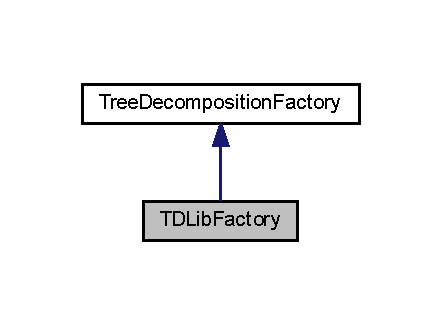
\includegraphics[width=212pt]{class_t_d_lib_factory__inherit__graph}
\end{center}
\end{figure}


Collaboration diagram for T\+D\+Lib\+Factory\+:\nopagebreak
\begin{figure}[H]
\begin{center}
\leavevmode
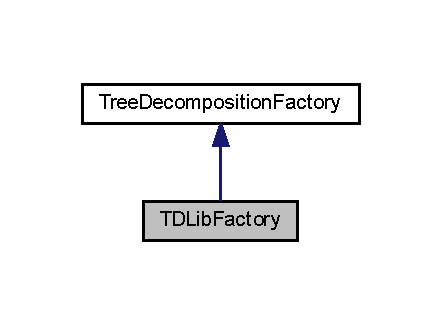
\includegraphics[width=212pt]{class_t_d_lib_factory__coll__graph}
\end{center}
\end{figure}
\subsection*{Public Member Functions}
\begin{DoxyCompactItemize}
\item 
\mbox{\Hypertarget{class_t_d_lib_factory_a7d8ce8a88978b4d5eca8bfd81a7ec030}\label{class_t_d_lib_factory_a7d8ce8a88978b4d5eca8bfd81a7ec030}} 
\hyperlink{class_tree_decomposition}{Tree\+Decomposition} $\ast$ {\bfseries make\+TD} (vector$<$ \hyperlink{class_secondary_structure}{Secondary\+Structure} $\ast$$>$ \&v)
\end{DoxyCompactItemize}


\subsection{Detailed Description}
The \hyperlink{class_t_d_lib_factory}{T\+D\+Lib\+Factory} class is a concrete implementation of \hyperlink{class_tree_decomposition_factory}{Tree\+Decomposition\+Factory} based on the T\+D\+Lib.\+jar Java implementation of the greedy fill-\/in heuristics. 

The documentation for this class was generated from the following files\+:\begin{DoxyCompactItemize}
\item 
src/Tree\+Decomposition.\+hpp\item 
src/Tree\+Decomposition.\+cpp\end{DoxyCompactItemize}

\hypertarget{class_tree_decomposition}{}\section{Tree\+Decomposition Class Reference}
\label{class_tree_decomposition}\index{Tree\+Decomposition@{Tree\+Decomposition}}
\subsection*{Public Member Functions}
\begin{DoxyCompactItemize}
\item 
\mbox{\Hypertarget{class_tree_decomposition_a4d68db24421f1c049b6535f760df01c1}\label{class_tree_decomposition_a4d68db24421f1c049b6535f760df01c1}} 
\hyperlink{class_tree_decomposition_a4d68db24421f1c049b6535f760df01c1}{Tree\+Decomposition} ()
\begin{DoxyCompactList}\small\item\em \hyperlink{class_tree_decomposition}{Tree\+Decomposition} Constructs an empty tree decomposition. \end{DoxyCompactList}\item 
vector$<$ \hyperlink{class_bag}{Bag} $\ast$ $>$ \hyperlink{class_tree_decomposition_a204777cf6460de25bc733a2fff4fb38c}{topological\+Sort} ()
\begin{DoxyCompactList}\small\item\em topological\+Sort Builds a topological ordering of bags \end{DoxyCompactList}\item 
void \hyperlink{class_tree_decomposition_abc2d6a2e7023ada23048b9a4832ef1b1}{load\+From\+File} (string path)
\begin{DoxyCompactList}\small\item\em load\+From\+File Loads the content of a tree-\/decomposition from a file \end{DoxyCompactList}\item 
void \hyperlink{class_tree_decomposition_acb7575c5835a306e72590fa755cb5009}{add\+Structure} (\hyperlink{class_secondary_structure}{Secondary\+Structure} $\ast$ss)
\begin{DoxyCompactList}\small\item\em add\+Structure Adds the structural elements of a secondary structure to the suitable bags in the tree-\/decomposition \end{DoxyCompactList}\item 
vector$<$ \hyperlink{class_bag}{Bag} $\ast$ $>$ \hyperlink{class_tree_decomposition_a91c0f9cf765260fe982c40fc17c29919}{get\+Bags} ()
\begin{DoxyCompactList}\small\item\em get\+Bags Returns the set of bags for this tree decomposition \end{DoxyCompactList}\item 
void \hyperlink{class_tree_decomposition_a328efa3fba52a273997eac5fe43083f3}{show} (int depth=0)
\begin{DoxyCompactList}\small\item\em show Prints this tree decomposition recursively to standard error \end{DoxyCompactList}\end{DoxyCompactItemize}
\subsection*{Public Attributes}
\begin{DoxyCompactItemize}
\item 
\mbox{\Hypertarget{class_tree_decomposition_ac5fd738f6c5c620a2b5935782aecc40f}\label{class_tree_decomposition_ac5fd738f6c5c620a2b5935782aecc40f}} 
vector$<$ \hyperlink{class_bag}{Bag} $\ast$ $>$ {\bfseries bags}
\item 
\mbox{\Hypertarget{class_tree_decomposition_a4eead3f83f7cdcb953618bd226a6ec6b}\label{class_tree_decomposition_a4eead3f83f7cdcb953618bd226a6ec6b}} 
vector$<$ int $>$ {\bfseries roots}
\end{DoxyCompactItemize}


\subsection{Member Function Documentation}
\mbox{\Hypertarget{class_tree_decomposition_acb7575c5835a306e72590fa755cb5009}\label{class_tree_decomposition_acb7575c5835a306e72590fa755cb5009}} 
\index{Tree\+Decomposition@{Tree\+Decomposition}!add\+Structure@{add\+Structure}}
\index{add\+Structure@{add\+Structure}!Tree\+Decomposition@{Tree\+Decomposition}}
\subsubsection{\texorpdfstring{add\+Structure()}{addStructure()}}
{\footnotesize\ttfamily void Tree\+Decomposition\+::add\+Structure (\begin{DoxyParamCaption}\item[{\hyperlink{class_secondary_structure}{Secondary\+Structure} $\ast$}]{ss }\end{DoxyParamCaption})}



add\+Structure Adds the structural elements of a secondary structure to the suitable bags in the tree-\/decomposition 


\begin{DoxyParams}{Parameters}
{\em ss} & Secondary structure to be added \\
\hline
\end{DoxyParams}
\mbox{\Hypertarget{class_tree_decomposition_a91c0f9cf765260fe982c40fc17c29919}\label{class_tree_decomposition_a91c0f9cf765260fe982c40fc17c29919}} 
\index{Tree\+Decomposition@{Tree\+Decomposition}!get\+Bags@{get\+Bags}}
\index{get\+Bags@{get\+Bags}!Tree\+Decomposition@{Tree\+Decomposition}}
\subsubsection{\texorpdfstring{get\+Bags()}{getBags()}}
{\footnotesize\ttfamily vector$<$ \hyperlink{class_bag}{Bag} $\ast$ $>$ Tree\+Decomposition\+::get\+Bags (\begin{DoxyParamCaption}{ }\end{DoxyParamCaption})}



get\+Bags Returns the set of bags for this tree decomposition 

\begin{DoxyReturn}{Returns}
List of pointers to bags in this tree decomposition 
\end{DoxyReturn}
\mbox{\Hypertarget{class_tree_decomposition_abc2d6a2e7023ada23048b9a4832ef1b1}\label{class_tree_decomposition_abc2d6a2e7023ada23048b9a4832ef1b1}} 
\index{Tree\+Decomposition@{Tree\+Decomposition}!load\+From\+File@{load\+From\+File}}
\index{load\+From\+File@{load\+From\+File}!Tree\+Decomposition@{Tree\+Decomposition}}
\subsubsection{\texorpdfstring{load\+From\+File()}{loadFromFile()}}
{\footnotesize\ttfamily void Tree\+Decomposition\+::load\+From\+File (\begin{DoxyParamCaption}\item[{string}]{path }\end{DoxyParamCaption})}



load\+From\+File Loads the content of a tree-\/decomposition from a file 


\begin{DoxyParams}{Parameters}
{\em path} & Path to a file describing a tree-\/decomposition \\
\hline
\end{DoxyParams}
\mbox{\Hypertarget{class_tree_decomposition_a328efa3fba52a273997eac5fe43083f3}\label{class_tree_decomposition_a328efa3fba52a273997eac5fe43083f3}} 
\index{Tree\+Decomposition@{Tree\+Decomposition}!show@{show}}
\index{show@{show}!Tree\+Decomposition@{Tree\+Decomposition}}
\subsubsection{\texorpdfstring{show()}{show()}}
{\footnotesize\ttfamily void Tree\+Decomposition\+::show (\begin{DoxyParamCaption}\item[{int}]{depth = {\ttfamily 0} }\end{DoxyParamCaption})}



show Prints this tree decomposition recursively to standard error 


\begin{DoxyParams}{Parameters}
{\em depth} & Depth in tree decomposition of current bag \\
\hline
\end{DoxyParams}
\mbox{\Hypertarget{class_tree_decomposition_a204777cf6460de25bc733a2fff4fb38c}\label{class_tree_decomposition_a204777cf6460de25bc733a2fff4fb38c}} 
\index{Tree\+Decomposition@{Tree\+Decomposition}!topological\+Sort@{topological\+Sort}}
\index{topological\+Sort@{topological\+Sort}!Tree\+Decomposition@{Tree\+Decomposition}}
\subsubsection{\texorpdfstring{topological\+Sort()}{topologicalSort()}}
{\footnotesize\ttfamily vector$<$ \hyperlink{class_bag}{Bag} $\ast$ $>$ Tree\+Decomposition\+::topological\+Sort (\begin{DoxyParamCaption}{ }\end{DoxyParamCaption})}



topological\+Sort Builds a topological ordering of bags 

\begin{DoxyReturn}{Returns}
List of topologically-\/sorted (leaves before internal, children before parent) bags 
\end{DoxyReturn}


The documentation for this class was generated from the following files\+:\begin{DoxyCompactItemize}
\item 
src/Tree\+Decomposition.\+hpp\item 
src/Tree\+Decomposition.\+cpp\end{DoxyCompactItemize}

\hypertarget{class_tree_decomposition_factory}{}\section{Tree\+Decomposition\+Factory Class Reference}
\label{class_tree_decomposition_factory}\index{Tree\+Decomposition\+Factory@{Tree\+Decomposition\+Factory}}


The \hyperlink{class_tree_decomposition_factory}{Tree\+Decomposition\+Factory} class is an abstract class aimed at producing a tree decomposition from a set of secondary structures.  




{\ttfamily \#include $<$Tree\+Decomposition.\+hpp$>$}



Inheritance diagram for Tree\+Decomposition\+Factory\+:\nopagebreak
\begin{figure}[H]
\begin{center}
\leavevmode
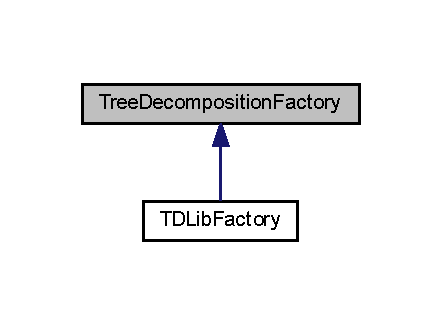
\includegraphics[width=212pt]{class_tree_decomposition_factory__inherit__graph}
\end{center}
\end{figure}
\subsection*{Public Member Functions}
\begin{DoxyCompactItemize}
\item 
\mbox{\Hypertarget{class_tree_decomposition_factory_a249cdde92245b4add19fafa00ad9be52}\label{class_tree_decomposition_factory_a249cdde92245b4add19fafa00ad9be52}} 
virtual \hyperlink{class_tree_decomposition}{Tree\+Decomposition} $\ast$ {\bfseries make\+TD} (vector$<$ \hyperlink{class_secondary_structure}{Secondary\+Structure} $\ast$$>$ \&v)=0
\end{DoxyCompactItemize}


\subsection{Detailed Description}
The \hyperlink{class_tree_decomposition_factory}{Tree\+Decomposition\+Factory} class is an abstract class aimed at producing a tree decomposition from a set of secondary structures. 

The documentation for this class was generated from the following file\+:\begin{DoxyCompactItemize}
\item 
src/Tree\+Decomposition.\+hpp\end{DoxyCompactItemize}

%--- End generated contents ---

% Index
\backmatter
\newpage
\phantomsection
\clearemptydoublepage
\addcontentsline{toc}{chapter}{Index}
\printindex

\end{document}
